\documentclass[border=5mm]{standalone}
\usepackage{tikz}
\usetikzlibrary{calc}           % For general calculations
\usetikzlibrary{matrix}         % For the matrix cmd
\usetikzlibrary{positioning}    % For above = Xcm of and similars
\usetikzlibrary{intersections}  % Mainly here for the arc over line
\usetikzlibrary{topaths}        % Enable move to operation
\usetikzlibrary{backgrounds}    % Put colors in background
\usetikzlibrary{shapes}         % Allow use of more shapes

\tikzset{rosnode/.style={ellipse,
                        fill=blue!20,
                        matrix of nodes,
                        row sep=1mm,
                        column sep=1mm,
                        nodes={anchor=center, inner sep=0pt, outer sep=0pt}
                        },
        rostopic/.style={ellipse,
                        fill=blue!50,
                        matrix of nodes,
                        row sep=1mm,
                        column sep=1mm,
                        nodes={anchor=center, inner sep=0pt, outer sep=0pt}
        },
}

\begin{document}
\sffamily

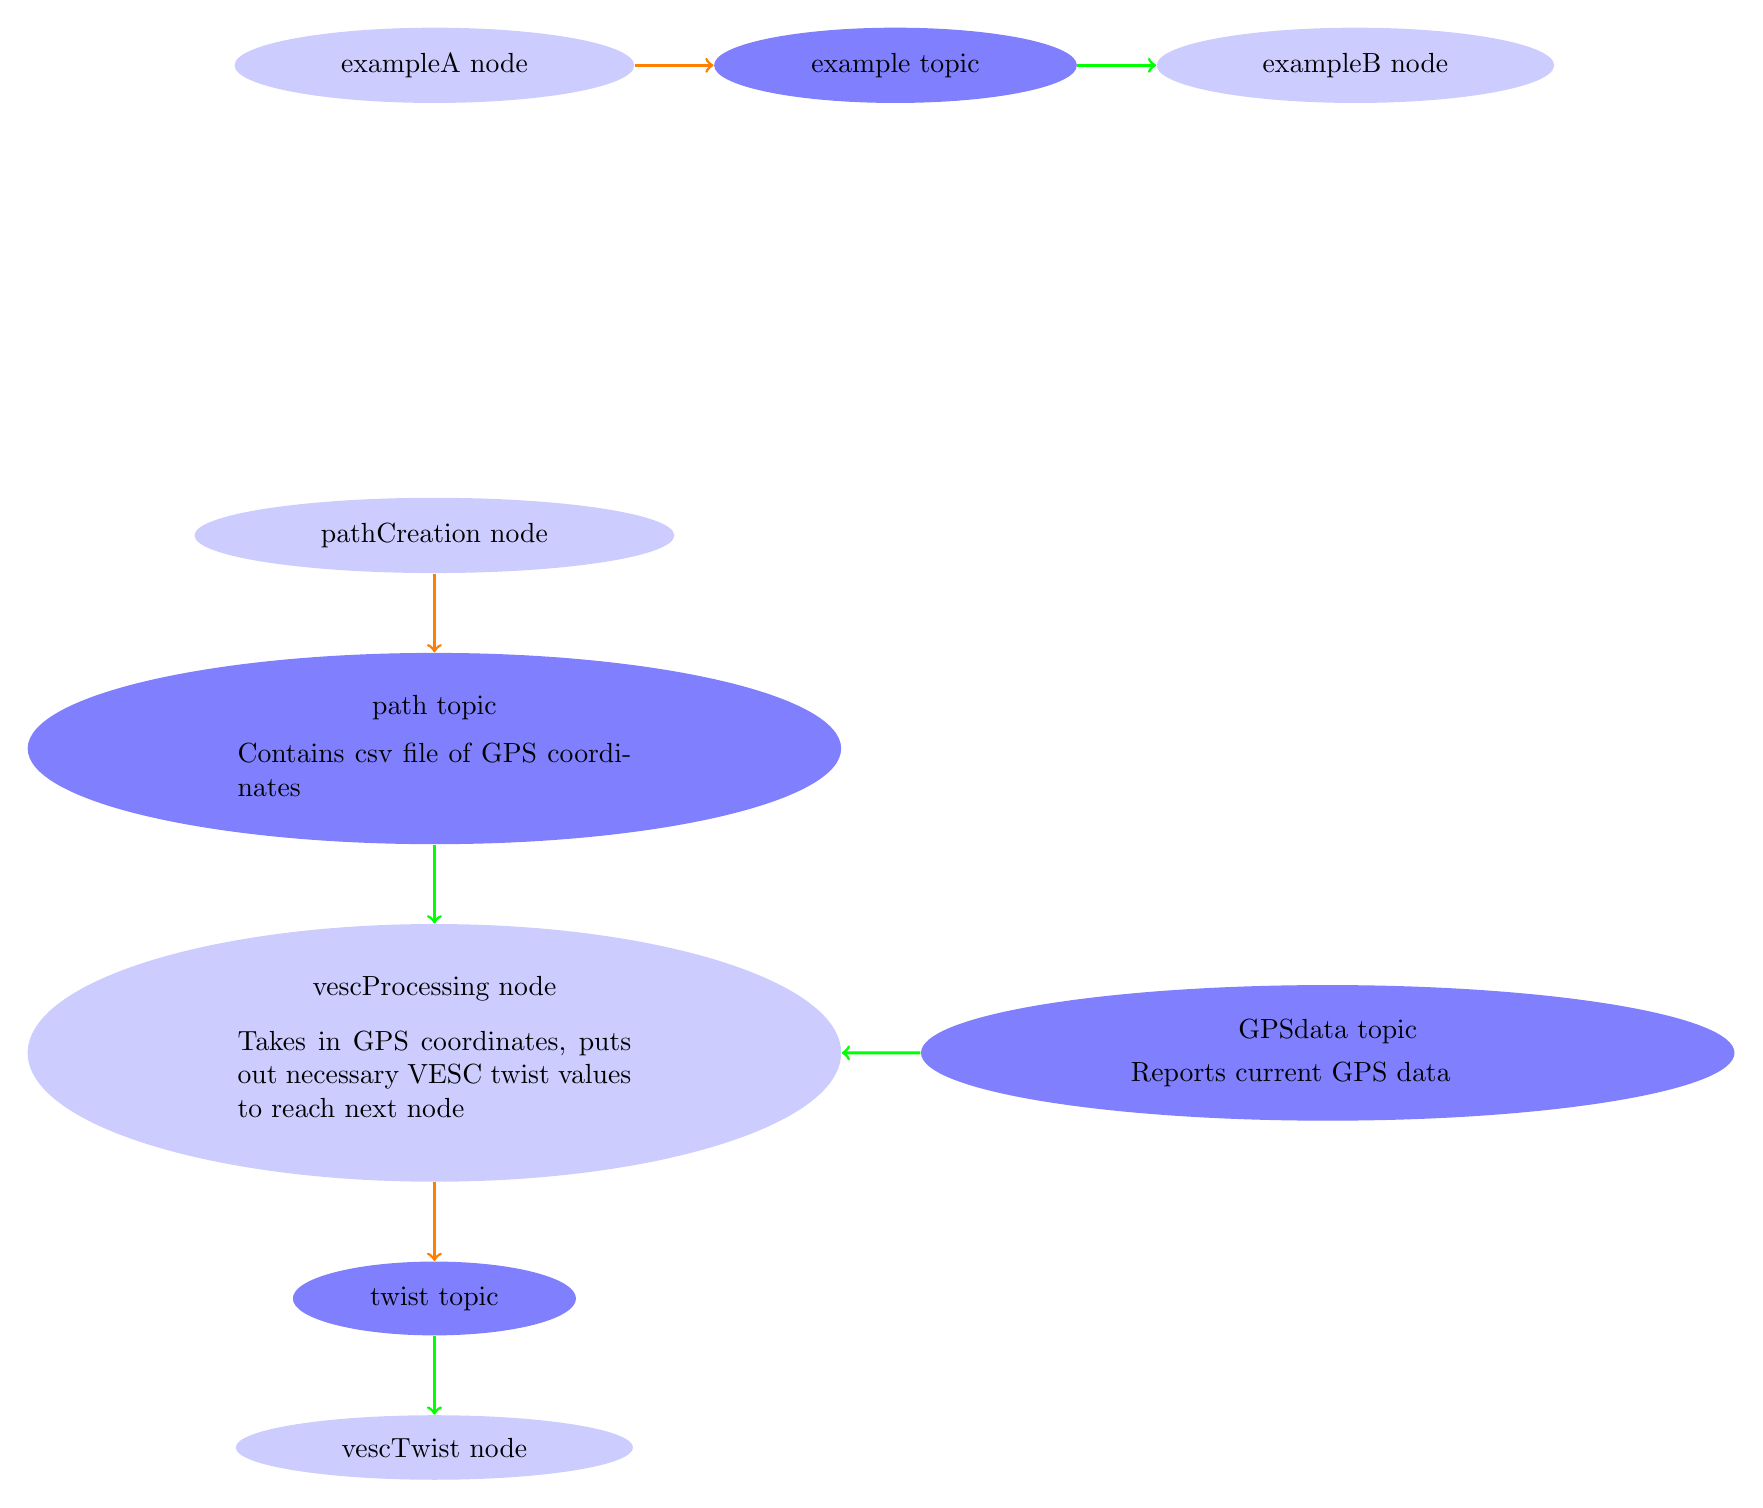
\begin{tikzpicture}
    [scale=.9,auto=center]

    % EXAMPLE
    \matrix[rosnode] (exampleA) {
        exampleA node \\
    };

    \matrix[rostopic, right= of exampleA] (exampleC) {
        example topic \\
    };

    \matrix[rosnode, right= of exampleC] (exampleB) {
        exampleB node \\
    };
    
    \draw[->,orange,line width=1pt] (exampleA) -- (exampleC);
    \draw[->,green,line width=1pt] (exampleC) -- (exampleB);


    % NODE DIAGRAM
    \matrix[rosnode, below= 5cm of exampleA] (pathCreation) {
        pathCreation node \\
    };

    \matrix[rostopic, below= of pathCreation] (path) {
        path topic \\
        \parbox{5cm}{Contains csv file of GPS coordinates} \\
    };

    \matrix[rosnode, below= of path] (vescProcessing) {
        vescProcessing node \\
        \parbox{5cm}{Takes in GPS coordinates, puts out necessary VESC twist values to reach next node} \\
    };

    \matrix[rostopic, right= of vescProcessing] (GPSdata) {
        GPSdata topic \\
        \parbox{5cm}{Reports current GPS data} \\
    };

    \matrix[rostopic, below= of vescProcessing] (twist) {
        twist topic \\
    };

    \matrix[rosnode, below= of twist] (vescTwist) {
        vescTwist node \\
    };
    
    \draw[->,orange,line width=1pt] (pathCreation) -- (path);
    \draw[->,green,line width=1pt] (path) -- (vescProcessing);
    \draw[->,green,line width=1pt] (GPSdata) -- (vescProcessing);
    \draw[->,orange,line width=1pt] (vescProcessing) -- (twist);
    \draw[->,green,line width=1pt] (twist) -- (vescTwist);
    
\end{tikzpicture}
\end{document}